We allow the spin-down, frequency, and phase to undergo a random walk such that
each step proceeds from the previous value and the steps themselves are
normally distributed. Constraining the spin-down to be the highest order term
allowed to vary we have
\begin{equation}
\Delta \fdot_{i} - \Delta\fdot_{i-1} = \tn \fdot_{i} \sim N(0, \sigS)
\end{equation}•
Notice that the residual between parameter space offsets is denoted by $\tn$
which is always normally distributed. Rearranging this gives an expression for
the offset in the $i^{th}$ segment, by induction we can also write down the
$i-1$ term
\begin{align}
\Delta\fdot_{i} &  = \tn\fdot_{i} + \Delta\fdot_{i-1}  \\
\Delta\fdot_{i-1} &  = \tn\fdot_{i-1} + \Delta\fdot_{i-2}  .
\end{align}
As each step proceeds from the previous step, and the random walk begins at the
origin, we can write
\begin{equation} 
\Delta\fdot_{i} = \s{j=1}{i}\tn\fdot_{j}.
\label{eqn: fdot offset} 
\end{equation}

If we want to build a realistic model, then we must consider the effect that a
random walk in spin-down may have on the frequency and phase. For example if we
increase the spin-down for a period of time, then we would expect the frequency
to decrease at a greater rate during this period. In our discreet model it is
not possible to dynamically change the frequency during a single segment.
However, we can approximate this by updating the frequency in the next
segment with the induced frequency offset due to the spin-down in previous
segments. This must be done for lower order terms for each random walk in the
frequency and spin-down. For the phase no lower order terms exist so there is no
induced effect.

Because the random walk is discreet and constant in any given segment, we can
calculate the offset in the lower order terms from a Taylor expansion. The
total offset at the  $i^{th}$ reference time is then given by the summation of
the offset caused by higher order terms up to that reference time. The reference times
can be arbitrarily chosen, but setting each to start at the beginning of the segment
simplifies the calculation.
In figure~\ref{fig: Illustration fdot int} we plot the random walk in spin-down as given by 
\eqref{eqn: fdot offset}. The frequency offset induced by the spin-down can be
calculated using a Taylor expansion
\begin{equation}
\Delta \f_{i} = \s{j=1}{i-1}\Delta\fdot_{j} \dT 
\label{eqn: f offset induced} 
\end{equation}

This can be though of as the integration of the spin-down up to the $i^{th}$
reference time and is illustrated by the shaded region in figure~\ref{fig:
Illustration fdot int}. 

\begin{figure}[ht]
\centering
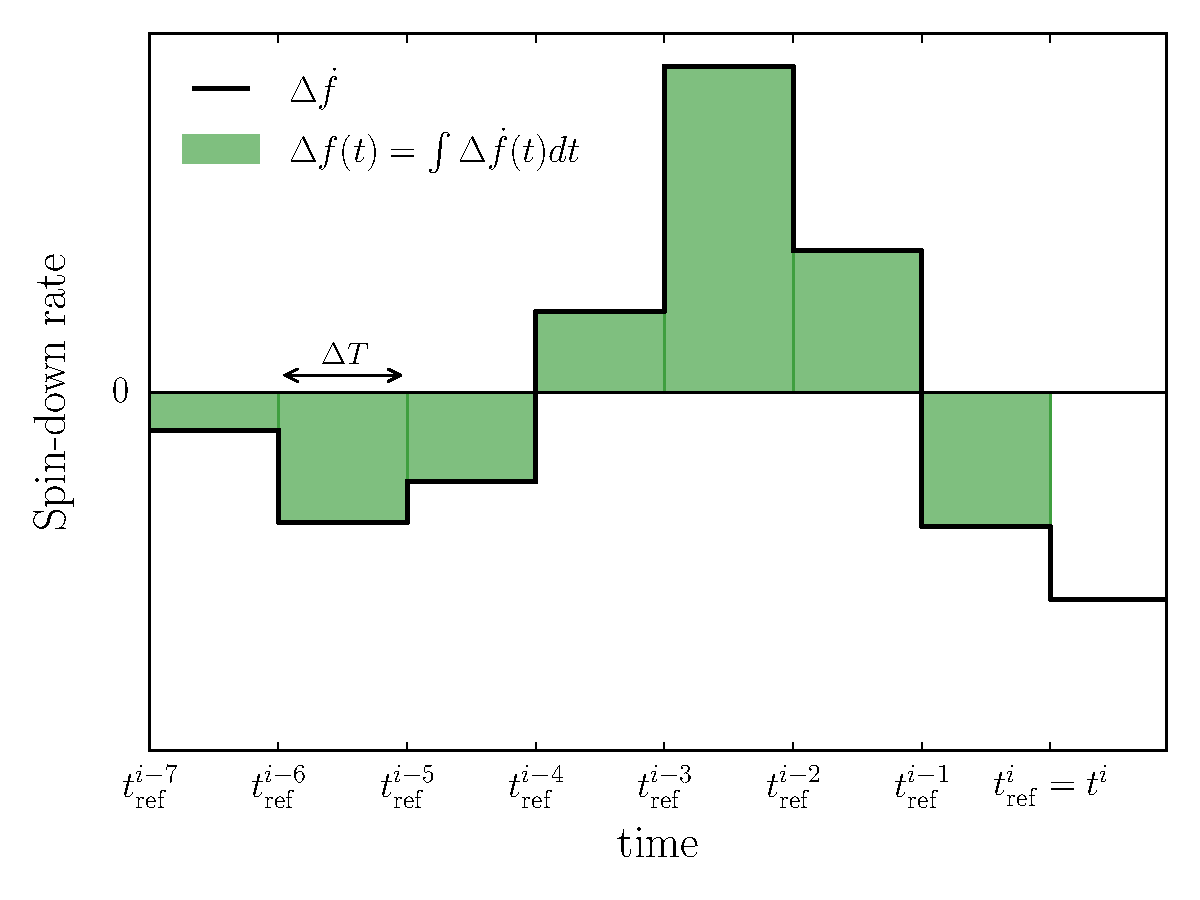
\includegraphics[width=0.7\textwidth]{Illustration_F1_int}
\caption{Illustration of equation~\eqref{eqn: f offset induced} demonstrating
a random walk in the spin-down and the filled in region which we
integrate over to find the frequency offset at $t_{i}$.}
\label{fig: Illustration fdot int}
\end{figure}

Since we want to consider random walks in all three parameters we now add in a
random walk in frequency. Each step is independent of the induced effect from
the spin-down and is given by \mbox{$\tn \f_{i} \sim N(0, \sigF)$}. The two
effects will sum linearly such that the frequency offset is
\begin{equation}
\Delta \f_{i} = \s{j=1}{i}\tn \f_{j} + \s{j=1}{i-1}\Delta\fdot_{j} \dT.
\label{eqn: f offset} 
\end{equation}•

By a similar process we can calculate the induced effect of the frequency and
spin-down on the phase. In full the phase offset is given by
\begin{equation}
\Delta\phi_{i}  =  \s{j=1}{i}\tn \phi_{j} 
+ 2\pi\left(\s{j=1}{i-1}\Delta \f_{j}\dT 
+ \frac{1}{2}\s{j=1}{i-1}\Delta \fdot_{j}\dT^{2}\right) \label{eqn: phi offset} 
\end{equation}

%Equations \eqref{eqn: f offset} and \eqref{eqn: phi offset} will allows us to
%construct the parameter space offsets in all three terms from the distibutions
%$\tn \phi_i$, $\tn \phi_i$, and $\tn \phi_i$.


